   
\documentclass[11pt]{article}
\renewcommand{\baselinestretch}{1.05}
\usepackage{amsmath,amsthm,verbatim,amssymb,amsfonts,amscd, graphicx}
\usepackage{mathtools}
\usepackage[table,xcdraw]{xcolor}
\DeclarePairedDelimiter{\ceil}{\lceil}{\rceil}
\usepackage{graphics}
\usepackage{enumitem}
\usepackage[table]{xcolor}
\usepackage{floatrow}
\usepackage{geometry}
\usepackage{tikz}
\usetikzlibrary{shapes.geometric,arrows,chains,fit,shapes,calc,matrix,positioning}
\tikzset
{
    treenode/.style = {rectangle, draw=black, align=center, minimum size=1cm},
    subtree/.style  = {isosceles triangle, draw=black, align=center, minimum height=0.5cm, minimum width=1cm, shape border rotate=90, anchor=north}
}
\topmargin0.0cm
\headheight0.0cm
\headsep0.0cm
\oddsidemargin0.0cm
\textheight23.0cm
\textwidth16.5cm
\footskip1.0cm
\theoremstyle{plain}

\definecolor{myblue}{RGB}{80,80,160}
\definecolor{mygreen}{RGB}{80,160,80}
\newtheorem{theorem}{Theorem}
\newtheorem{corollary}{Corollary}
\usepackage{clrscode}
\newtheorem{lemma}{Lemma}
\newtheorem{proposition}{Proposition}
\newtheorem*{surfacecor}{Corollary 1}
\newtheorem{conjecture}{Conjecture} 
\newtheorem{question}{Question} 
\theoremstyle{definition}
\newtheorem{definition}{Definition}

\newlist{pcases}{enumerate}{1}
\setlist[pcases]{
  label=\underline{Case~\arabic*:}\protect\thiscase.~,
  ref=\arabic*,
  align=left,
  labelsep=0pt,
  leftmargin=0pt,
  labelwidth=0pt,
  parsep=0pt
}
\newcommand{\case}[1][]{%
  \if\relax\detokenize{#1}\relax
    \def\thiscase{}%
  \else
    \def\thiscase{~#1}%
  \fi
  \item
}
\usepackage{listings}
\usepackage{color}

\definecolor{dkgreen}{rgb}{0,0.6,0}
\definecolor{gray}{rgb}{0.5,0.5,0.5}
\definecolor{mauve}{rgb}{0.58,0,0.82}

\lstset{frame=tb,
  language=Java,
  aboveskip=3mm,
  belowskip=3mm,
  showstringspaces=false,
  columns=flexible,
  basicstyle={\small\ttfamily},
  numbers=none,
  numberstyle=\tiny\color{gray},
  keywordstyle=\color{blue},
  commentstyle=\color{dkgreen},
  stringstyle=\color{mauve},
  breaklines=true,
  breakatwhitespace=true
  tabsize=3
}
\newcommand{\blank}[1]{\hfil\penalty1000\hfilneg\rule[-3pt]{#1}{0.4pt}}
\begin{document}
 


\title{Introduction to Flow Networks}
\author{By Joshua Kirstein (joshkirstein@ufl.edu)}
\maketitle

\section{Introduction}
Just like how most of Graph Theory is motivated by real world examples, so will today's set of lecture notes. Imagine a system of interconnected pipes starting at your sink and ending in the sewer. Each pipe can only hold a certain amount of water, and we'd like to model the flow of water from when you turn on the faucet to when the water eventually reaches the sewer. In order to abstract the notion of flowing water and pipes with capacity away, we will design a new type of graph called \emph{flow networks}. After we have designed the machinery allowing us to consider problems that can be described as a flow network, we will design an algorithm to compute the so-called \emph{maximum flow} (abbreviated by `max-flow') of a given flow network: the maximum amount of water that can flow from the sink to the sewer at any given point. A surprising duality between the max-flow problem will be established shortly after.\\\\
It is important to note that max-flow is almost never used in its raw form. Just like you're able to solve the problem of finding the intersection of two circles (geometric interpretation) using the quadratic formula (algebraic interpretation), we'll show that a surprising number of different problems can be solved by interpreting them as max-flow problems. As a side note: this idea of interpreting a problem (intersection of two circles vs. quadratic formula) from a new vantage point is called `reduction'; that is, we've reduced the problem of finding the intersection points of two circles to a simple use of the quadratic formula.\\\\
To safely breeze through these notes you should be familiar with basic graph theory (the notions of vertices, edges, un-weighted/weighted graphs, un-directed/directed graphs, acyclic/cyclic graphs, breadth-first search, etc).
\section{Flow Networks}

We'll start our discussion by first putting notation to the situation described in the introduction. To that end, we'll introduce the ideas of \emph{flow networks} and \emph{flows}. Flow networks will give us a way to describe the constraints in the environment (pipe capacities, connection between pipes) and flows will give us a way to describe water actually flowing through one of these networks. A \emph{flow network} is just a weighted directed graph that is imbued with a `source' and `sink' node; the edge weights are interpreted as `pipe capacities' while the source and sink nodes are interpreted as the start and end of the flow of water (remember, flow networks is just a tool we'll be using to describe an environment that can have `water flow'). Throughout these lecture notes we will denote the source of a flow network by `s' and the sink by `t'; it is by convention that we draw the `source' node on the left side of the graph and the `sink' node on the right side.  A few examples of flow networks are provided below.
\begin{figure}[h]
\caption{An example flow network.}
\centering
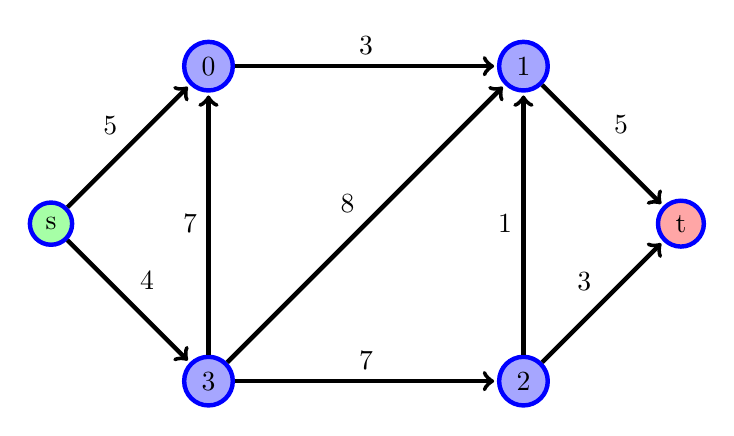
\begin{tikzpicture}[shorten >=1pt, auto, node distance=3cm, ultra thick]
   \begin{scope}[every node/.style={circle,draw=blue,fill=blue!35!}]
    \node (v1) at (-2,2) {0};
    \node (v2) at (2,2) {1};
    \node (v3) [fill=red!35!] at (4,0) {t};
    \node (v4) at (2,-2) {2};
    \node (v5) at (-2,-2) {3};
    \node (v6) [fill=green!35!] at (-4,0) {s};
   \end{scope}
   \begin{scope}[->,every edge/.style={draw=black,ultra thick}]
    \draw  (v1) edge node{3} (v2);
    \draw  (v2) edge node{5} (v3);
    \draw  (v4) edge node{3} (v3);
    \draw  (v5) edge node{7} (v4);
    \draw  (v6) edge node{4} (v5);
    \draw  (v6) edge node{5} (v1);
    \draw  (v5) edge node{7} (v1);
    \draw  (v5) edge node{8} (v2);
    \draw  (v4) edge node{1} (v2);
   \end{scope}
\end{tikzpicture}
\end{figure}

\noindent It is possible to have two edges associated with a pair of vertices, and this is interpreted as having two distinct pipes that allow flow in opposite directions.
\begin{figure}[h]
\caption{An example flow network that allows bidirectional flow on a pair of vertices.}
\centering
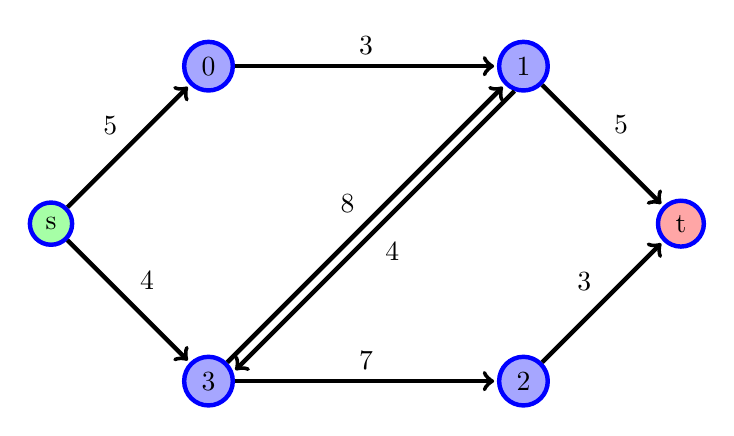
\begin{tikzpicture}[shorten >=1pt, auto, node distance=3cm, ultra thick]
   \begin{scope}[every node/.style={circle,draw=blue,fill=blue!35!}]
    \node (v1) at (-2,2) {0};
    \node (v2) at (2,2) {1};
    \node (v3) [fill=red!35!] at (4,0) {t};%keeping track of current flow assignment
%look at residual graph
%find a path in residual graph
%augment!
    \node (v4) at (2,-2) {2};
    \node (v5) at (-2,-2) {3};
    \node (v6) [fill=green!35!] at (-4,0) {s};
   \end{scope}
   \begin{scope}[->,every edge/.style={draw=black,ultra thick}]
    \draw  (v1) edge node{3} (v2);
    \draw  (v2) edge node{5} (v3);
    \draw  (v4) edge node{3} (v3);
    \draw  (v5) edge node{7} (v4);
    \draw  (v6) edge node{4} (v5);
    \draw  (v6) edge node{5} (v1);
    \draw  (v5) edge node{8} (v2);
    \draw  (v2.-110) -- node{4} (v5.20);
   \end{scope}
\end{tikzpicture}
\end{figure}
It should be obvious that any flow network can be represented (in memory) just like any other weighted, directed graph, except we need to be careful and identify which node is the source and which is the sink. In practice, flow networks are implemented via adjacency lists since they tend to have many nodes and relatively few edges.
\section{Valid Flow Assignments}
Currently our view of flow networks is sort of incomplete: how do we model actual water flowing through this network? For this we will introduce the concept of flows, which will correspond with a `snapshot' of how much water is in each pipe at any given time. Going from this raw physical idea to a refined conceptual idea is sort of tricky since we need to be careful and define the rule of how water flow can look like in our flow network. Clearly we don't want more water going through edges than their capacities allow. Additionally, if 30 water flows into some vertex, we can't really expect 40 water to come out (water doesn't appear out of thin air!). We will take care of these corner cases when defining flows. It is also important to keep in mind that we are modeling water flowing from the `source' to the `sink'. The `source' can give it as much water as necessary and the `sink' can take in as much water as the edges coming into it allow; this effectively tells us that the only `constraints' in our flow network are the capacities of the edges and the connections they define.\\\\
So what is \emph{flow} anyway? Simply put, it's just an assignment of values to each edge denoting how much flow (read: water) is going through that edge. For notational convenience, we say that the flow going from node $u$ to node $v$ is just the value $f(u, v)$; additionally, we say the capacity of the edge from node $u$ to node $v$ is $c(u, v)$. The discussion above gave examples of the complexities that we need to account for in order for a particular assignment of flow values to be valid, and we address them now. A flow is \emph{valid} if all of these conditions are satisfied:
\\\\
(1) (Capacity constraint) For all edges $(u, v)$, $0 \leq f(u, v) \leq c(u, v)$. All this says is that the flow going through an edge can't be larger than the capacity of that edge and flow is a positive value.
\\\\\
(2) (Flow conservation) For every node $u$ (except for the source and sink), $\sum_{v \neq u}{f(u, v)} = \sum_{v \neq u}{f(v, u)}$. Although the notation may seem scary, all it says is that the amount of flow coming into each node (the left hand side) is equal to the amount of flow coming out (the right hand side); it is important to note that this \emph{doesn't} apply for the source and sink, since there is no amount of flow going into the source and no amount of flow coming out of the sink.
\\\\
Note that you may often see different conditions depending on the literature that you read. The formulation we use above is called the \emph{positive flow formulation} and, although it's harder to use to prove properties about flows, it is \emph{much} easier think about and use when coding. At the end of the day, every formulation of flow is the same. We use the format $f / c$ to denote the flow and capacity of an edge (for example if an edge has capacity $5$ but $2$ flow going through it, we write $2/5$).
\\\\
Let's take a look at a couple of \emph{valid} and \emph{invalid} flows. Notice how in every case of \emph{valid} flow, the conditions stated above are satisfied and in every case of \emph{invalid} flow at least one isn't satisfied.
\begin{figure}[!ht]
\caption{An example of valid flow in a flow network.}
\centering
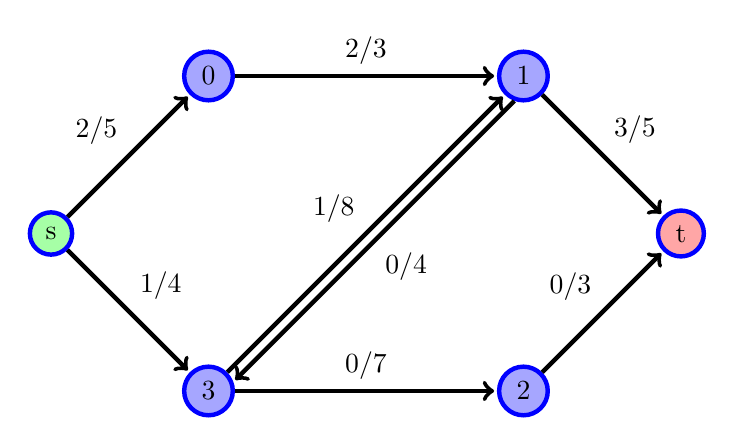
\begin{tikzpicture}[shorten >=1pt, auto, node distance=3cm, ultra thick]
   \begin{scope}[every node/.style={circle,draw=blue,fill=blue!35!}]
    \node (v1) at (-2,2) {0};
    \node (v2) at (2,2) {1};
    \node (v3) [fill=red!35!] at (4,0) {t};
    \node (v4) at (2,-2) {2};
    \node (v5) at (-2,-2) {3};
    \node (v6) [fill=green!35!] at (-4,0) {s};
   \end{scope}
   \begin{scope}[->,every edge/.style={draw=black,ultra thick}]
    \draw  (v1) edge node{2/3} (v2);
    \draw  (v2) edge node{3/5} (v3);
    \draw  (v4) edge node{0/3} (v3);
    \draw  (v5) edge node{0/7} (v4);
    \draw  (v6) edge node{1/4} (v5);
    \draw  (v6) edge node{2/5} (v1);
    \draw  (v5) edge node{1/8} (v2);
    \draw  (v2.-110) -- node{0/4} (v5.20);
   \end{scope}
\end{tikzpicture}
\end{figure}
\\
\begin{figure}[!ht]
\label{fig:maxflow1}
\caption{Another example of valid flow in a flow network. Notice how it's not possible to send flow anymore from the source to the sink.}
\centering
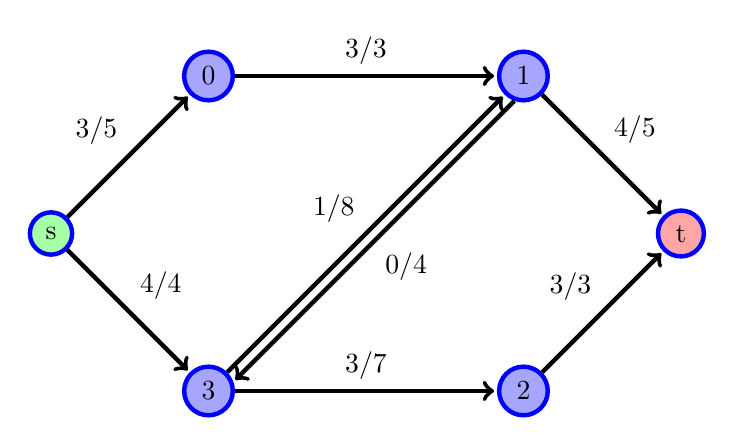
\begin{tikzpicture}[shorten >=1pt, auto, node distance=3cm, ultra thick]
   \begin{scope}[every node/.style={circle,draw=blue,fill=blue!35!}]
    \node (v1) at (-2,2) {0};
    \node (v2) at (2,2) {1};
    \node (v3) [fill=red!35!] at (4,0) {t};
    \node (v4) at (2,-2) {2};
    \node (v5) at (-2,-2) {3};
    \node (v6) [fill=green!35!] at (-4,0) {s};
   \end{scope}
   \begin{scope}[->,every edge/.style={draw=black,ultra thick}]
    \draw  (v1) edge node{3/3} (v2);
    \draw  (v2) edge node{4/5} (v3);
    \draw  (v4) edge node{3/3} (v3);
    \draw  (v5) edge node{3/7} (v4);
    \draw  (v6) edge node{4/4} (v5);
    \draw  (v6) edge node{3/5} (v1);
    \draw  (v5) edge node{1/8} (v2);
    \draw  (v2.-110) -- node{0/4} (v5.20);
   \end{scope}
\end{tikzpicture}
\end{figure}
\\
\begin{figure}[!ht]
\caption{An example of invalid flow in a flow network. Notice how nodes $1$ and $3$ violate the flow conservation property.}
\centering
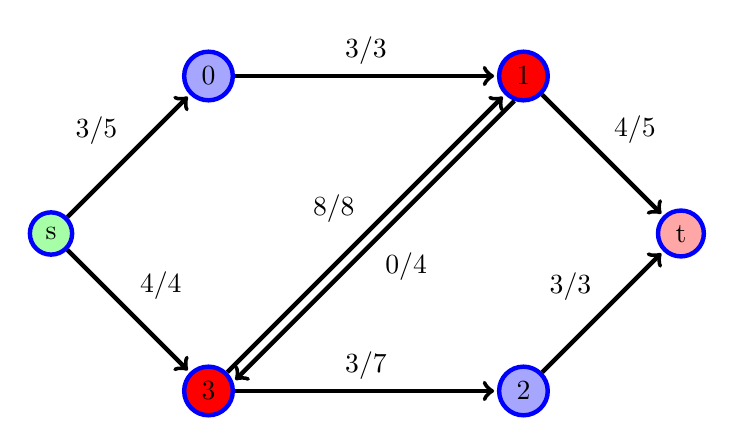
\begin{tikzpicture}[shorten >=1pt, auto, node distance=3cm, ultra thick]
   \begin{scope}[every node/.style={circle,draw=blue,fill=blue!35!}]
    \node (v1) at (-2,2) {0};
    \node (v2) [fill=red] at (2,2) {1};
    \node (v3) [fill=red!35!] at (4,0) {t};
    \node (v4) at (2,-2) {2};
    \node (v5) [fill=red] at (-2,-2) {3};
    \node (v6) [fill=green!35!] at (-4,0) {s};
   \end{scope}
   \begin{scope}[->,every edge/.style={draw=black,ultra thick}]
    \draw  (v1) edge node{3/3} (v2);
    \draw  (v2) edge node{4/5} (v3);
    \draw  (v4) edge node{3/3} (v3);
    \draw  (v5) edge node{3/7} (v4);
    \draw  (v6) edge node{4/4} (v5);
    \draw  (v6) edge node{3/5} (v1);
    \draw  (v5) edge node{8/8} (v2);
    \draw  (v2.-110) -- node{0/4} (v5.20);
   \end{scope}
\end{tikzpicture}
\end{figure}

\begin{figure}[!ht]
\caption{Another example of invalid flow in a flow network. Notice how the two red edges have more flow than their capacities allow.}
\centering
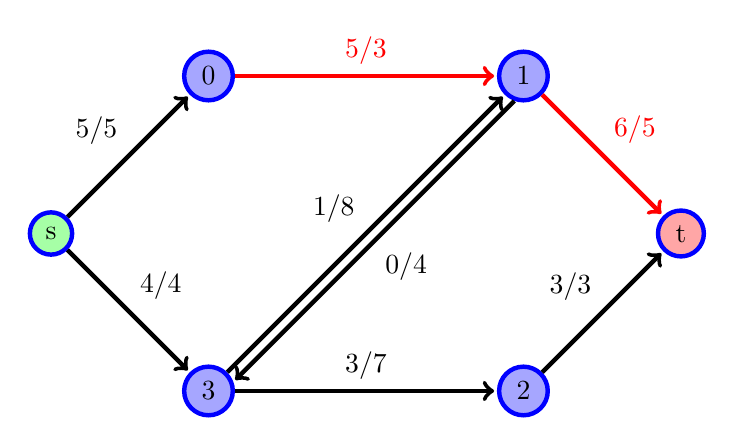
\begin{tikzpicture}[shorten >=1pt, auto, node distance=3cm, ultra thick]
   \begin{scope}[every node/.style={circle,draw=blue,fill=blue!35!}]
    \node (v1) at (-2,2) {0};
    \node (v2) at (2,2) {1};
    \node (v3) [fill=red!35!] at (4,0) {t};
    \node (v4) at (2,-2) {2};
    \node (v5) at (-2,-2) {3};
    \node (v6) [fill=green!35!] at (-4,0) {s};
   \end{scope}
   \begin{scope}[->,every edge/.style={draw=black,ultra thick}]
    \draw  (v1) edge[red] node{5/3} (v2);
    \draw  (v2) edge[red] node{6/5} (v3);
    \draw  (v4) edge node{3/3} (v3);
    \draw  (v5) edge node{3/7} (v4);
    \draw  (v6) edge node{4/4} (v5);
    \draw  (v6) edge node{5/5} (v1);
    \draw  (v5) edge node{1/8} (v2);
    \draw  (v2.-110) -- node{0/4} (v5.20);
   \end{scope}
\end{tikzpicture}
\end{figure}
\section{Computing the Largest Valid Flow Assignment}
At this point you should be familiar (conceptually) with what flow networks and valid flows are. In particular, you may have noticed in figure \ref{fig:maxflow1} it's physically impossible to allow anymore flow to go from the source to the sink. In this case we say that the flow has achieved a \emph{maximum value}, or is a \emph{maximum flow}. Specifically, a \emph{maximum flow} is a valid flow which, out of every possible valid flow, pushes the most amount of flow into the sink; we denote the `value' of a flow by $|f^*|$, which is just the amount of flow that $f$ pushes into the sink. 
\subsection{The idea of incrementally adding flow}
%basic idea is to just continue to push flow from source to sink
%if we can't push anymore flow, then we've reached the maximum flow
%look at the idea of redirected/backward flow (if we push flow along a bad path)
But how do we compute a maximum flow? We're going to first introduce all of the conceptual ideas required, so don't be afraid if you're not sure how to code anything until you finish the section on implementing these ideas. The basic idea behind almost every algorithm for computing the maximum flow is to continually find a path from the source to the sink which we can use to send flow between them; clearly the path must permit flow (the edges on the path can't be filled to capacity). Consider the following sequence of graphs.

\begin{figure}[!ht]
\caption{Initially we start with no flow along all of the edges.}
\centering
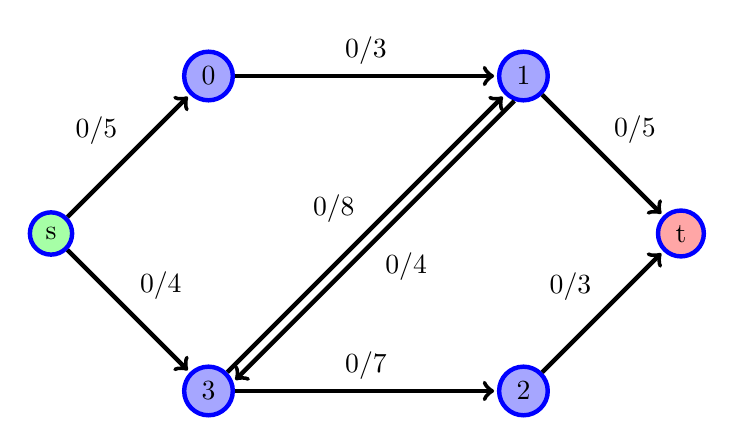
\begin{tikzpicture}[shorten >=1pt, auto, node distance=3cm, ultra thick]
   \begin{scope}[every node/.style={circle,draw=blue,fill=blue!35!}]
    \node (v1) at (-2,2) {0};
    \node (v2) at (2,2) {1};
    \node (v3) [fill=red!35!] at (4,0) {t};
    \node (v4) at (2,-2) {2};
    \node (v5) at (-2,-2) {3};
    \node (v6) [fill=green!35!] at (-4,0) {s};
   \end{scope}
   \begin{scope}[->,every edge/.style={draw=black,ultra thick}]
    \draw  (v1) edge node{0/3} (v2);
    \draw  (v2) edge node{0/5} (v3);
    \draw  (v4) edge node{0/3} (v3);
    \draw  (v5) edge node{0/7} (v4);
    \draw  (v6) edge node{0/4} (v5);
    \draw  (v6) edge node{0/5} (v1);
    \draw  (v5) edge node{0/8} (v2);
    \draw  (v2.-110) -- node{0/4} (v5.20);
   \end{scope}
\end{tikzpicture}
\end{figure}

\noindent Starting with no flow going from the source to the sink, we search for paths that allow us to push flow to the sink.

\begin{figure}[!ht]
\caption{We've found a path which permits flow, and so now we `augment' this path (add the flow it allows in).}
\centering
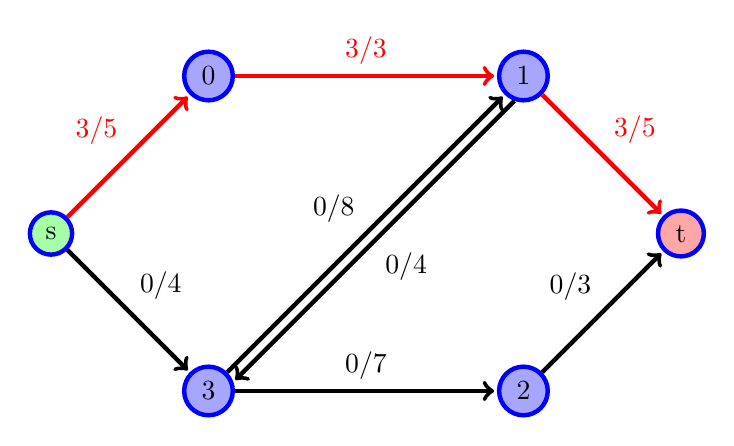
\begin{tikzpicture}[shorten >=1pt, auto, node distance=3cm, ultra thick]
   \begin{scope}[every node/.style={circle,draw=blue,fill=blue!35!}]
    \node (v1) at (-2,2) {0};
    \node (v2) at (2,2) {1};
    \node (v3) [fill=red!35!] at (4,0) {t};
    \node (v4) at (2,-2) {2};
    \node (v5) at (-2,-2) {3};
    \node (v6) [fill=green!35!] at (-4,0) {s};
   \end{scope}
   \begin{scope}[->,every edge/.style={draw=black,ultra thick}]
    \draw  (v1) edge [red] node{3/3} (v2);
    \draw  (v2) edge [red] node{3/5} (v3);
    \draw  (v4) edge node{0/3} (v3);
    \draw  (v5) edge node{0/7} (v4);
    \draw  (v6) edge node{0/4} (v5);
    \draw  (v6) edge [red] node{3/5} (v1);
    \draw  (v5) edge node{0/8} (v2);
    \draw  (v2.-110) -- node{0/4} (v5.20);
   \end{scope}
\end{tikzpicture}
\end{figure}

\noindent Here we have found a path colored in red and we `augment' the flow along this path. Since the smallest capacity on this path is $3$, that's how much flow we're allowed to send along this path.

\begin{figure}[!ht]
\caption{We've found \emph{another} path which permits flow.}
\centering
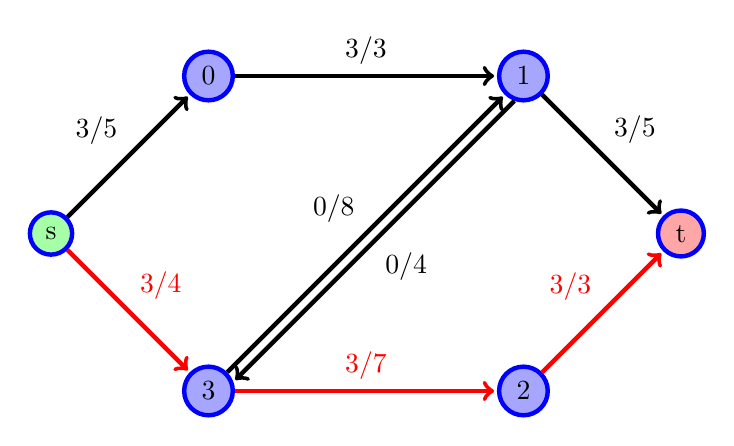
\begin{tikzpicture}[shorten >=1pt, auto, node distance=3cm, ultra thick]
   \begin{scope}[every node/.style={circle,draw=blue,fill=blue!35!}]
    \node (v1) at (-2,2) {0};
    \node (v2) at (2,2) {1};
    \node (v3) [fill=red!35!] at (4,0) {t};
    \node (v4) at (2,-2) {2};
    \node (v5) at (-2,-2) {3};
    \node (v6) [fill=green!35!] at (-4,0) {s};
   \end{scope}
   \begin{scope}[->,every edge/.style={draw=black,ultra thick}]
    \draw  (v1) edge node{3/3} (v2);
    \draw  (v2) edge node{3/5} (v3);
    \draw  (v4) edge [red] node{3/3} (v3);
    \draw  (v5) edge [red] node{3/7} (v4);
    \draw  (v6) edge [red] node{3/4} (v5);
    \draw  (v6) edge node{3/5} (v1);
    \draw  (v5) edge node{0/8} (v2);
    \draw  (v2.-110) -- node{0/4} (v5.20);
   \end{scope}
\end{tikzpicture}
\end{figure}
\newpage
\noindent We do the same with the next path that we find. Now the amount of flow being sent from the source to the sink is $3+3 = 6$; can we do better? There is one more path that we can augment:

\begin{figure}[!ht]
\caption{We've found the last path which permits flow.}
\centering
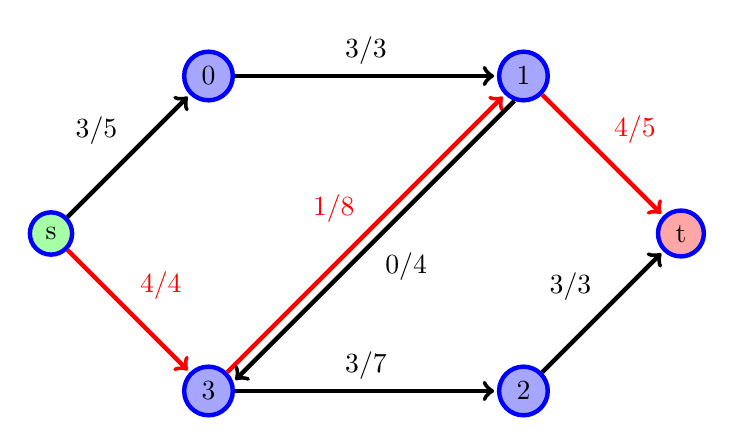
\begin{tikzpicture}[shorten >=1pt, auto, node distance=3cm, ultra thick]
   \begin{scope}[every node/.style={circle,draw=blue,fill=blue!35!}]
    \node (v1) at (-2,2) {0};
    \node (v2) at (2,2) {1};
    \node (v3) [fill=red!35!] at (4,0) {t};
    \node (v4) at (2,-2) {2};
    \node (v5) at (-2,-2) {3};
    \node (v6) [fill=green!35!] at (-4,0) {s};
   \end{scope}
   \begin{scope}[->,every edge/.style={draw=black,ultra thick}]
    \draw  (v1) edge node{3/3} (v2);
    \draw  (v2) edge [red] node{4/5} (v3);
    \draw  (v4) edge node{3/3} (v3);
    \draw  (v5) edge node{3/7} (v4);
    \draw  (v6) edge [red] node{4/4} (v5);
    \draw  (v6) edge node{3/5} (v1);
    \draw  (v5) edge [red] node{1/8} (v2);
    \draw  (v2.-110) -- node{0/4} (v5.20);
   \end{scope}
\end{tikzpicture}
\end{figure}

\noindent This last path only allows us to augment a flow of $1$ along it --- why? Now, no paths are left with which we can augment and thus we have achieved the maximum flow of $7$.\\

\noindent Okay perfect. So now we have our algorithm:
\\\\
\noindent (1) use bfs/dfs to find a path between the source and the sink that permits flow along it\\
(2) add the flow corresponding to that path to the graph\\
(3) repeat step (1) until no path exists\\

\noindent Right?
\newpage

\noindent Well we've got a slight problem. Consider the graph below. It should be clear that the maximum flow of it is $4$. But what happens if step (1) of our algorithm tries to augment this path:

\begin{figure}[!ht]
\label{fig:bad}
\caption{BAD PATH.}
\centering
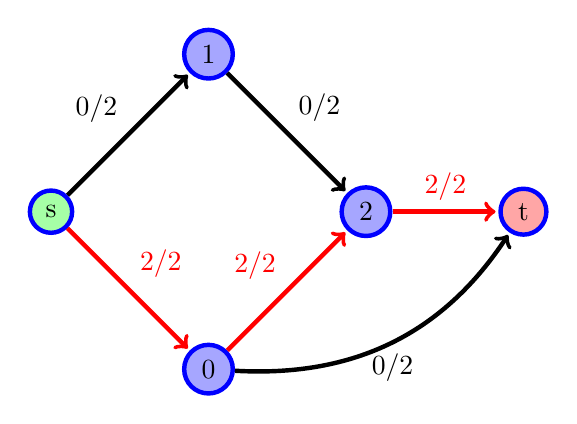
\begin{tikzpicture}[shorten >=1pt, auto, node distance=3cm, ultra thick]
   \begin{scope}[every node/.style={circle,draw=blue,fill=blue!35!}]
    \node (v1) [fill=green!35!]  at (0,2) {s};
    \node (v2) [fill=red!35!] at (6,2) {t};
    \node (v3) at (2,0) {0};
    \node (v4) at (2,4) {1};
    \node (v5) at (4,2) {2};
   \end{scope}
   \begin{scope}[->,every edge/.style={draw=black,ultra thick}]
    \draw  (v1) edge [red] node{2/2} (v3);    
    \draw  (v1) edge node{0/2} (v4);
    \draw  (v3) edge [red] node{2/2} (v5);
    \draw  (v4) edge node{0/2} (v5);
    \draw  (v5) edge [red] node{2/2} (v2);
    \draw  (v3) edge [bend right, below] node{0/2} (v2);
   \end{scope}
\end{tikzpicture}
\end{figure}

\noindent At this point, there are no other paths that will let us send flow from the source to the sink and thus our algorithm will report a maximum flow of $2$, which is incorrect. Our algorithm as we wrote it is currently incorrect. In the next section, we'll introduce the concept of a \emph{residual graph} which will help us undo flow that we send along a `bad path' as in figure \ref{fig:bad}.
\\\\
\noindent For now just notice that if we `reverse' the flow along edge $(0 \rightarrow 2)$ in the following path:
\begin{figure}[!ht]
\label{fig:bad}
\caption{The flow along edge $(0 \rightarrow 2)$ is reversed.}
\centering
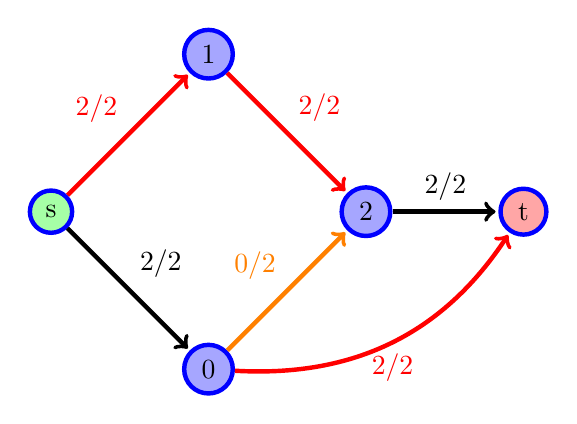
\begin{tikzpicture}[shorten >=1pt, auto, node distance=3cm, ultra thick]
   \begin{scope}[every node/.style={circle,draw=blue,fill=blue!35!}]
    \node (v1) [fill=green!35!]  at (0,2) {s};
    \node (v2) [fill=red!35!] at (6,2) {t};
    \node (v3) at (2,0) {0};
    \node (v4) at (2,4) {1};
    \node (v5) at (4,2) {2};
   \end{scope}
   \begin{scope}[->,every edge/.style={draw=black,ultra thick}]
    \draw  (v1) edge node{2/2} (v3);    
    \draw  (v1) edge [red] node{2/2} (v4);
    \draw  (v3) edge [orange] node{0/2} (v5);
    \draw  (v4) edge [red] node{2/2} (v5);
    \draw  (v5) edge node{2/2} (v2);
    \draw  (v3) edge [red, bend right, below] node{2/2} (v2);
   \end{scope}
\end{tikzpicture}
\end{figure}
\\
...that is, instead of adding $+2$ to the orange edge's flow, we add $-2$, then the resulting flow is indeed the maximum. This idea of reversing flow along some edges on a path is what powers residual graphs, as you will soon see.
\subsection{Cue Residual Graphs}
As we saw in the previous section, it's possible to find a path of edges from the source to the sink that leads us to a situation where we can't push any more flow, even though we haven't achieved the maximum flow. We're going to leverage the idea that we were starting to form at the end of the last section in order to get a correct algorithm. First, we will go over the specifics of what a \emph{residual graph} is and then demonstrate its correctness.\\\\
Let's go with the idea that we started with last section. Our idea was to have an incremental algorithm which would continually try and find a way to push flow from the source to the sink, push that flow, and then try again until it couldn't anymore. Given the current flow going through each edge, we're going to construct a new graph which will help us find these paths --- the \emph{residual graph}. The nodes in the residual graph correspond to the nodes in the original flow network; however, the edges are different. \\\\
For each edge in the original flow network we will construct two edges in the residual graph:
\\\\
(1) A \emph{forward edge} --- the forward edge is in the same direction as the original edge, except the weight of the edge is $({capacity}_{edge} - {flow}_{edge})$. Note that this value is called the \emph{residual capacity} of the edge and it represents the amount of flow that can be sent along this edge.
\\\\
(2) A \emph{reverse edge} --- the reverse edge is in the \emph{opposite} direction as the original edge, with weight equal to the amount of flow that is being sent along the residual edge. Just as in the previous section, this is supposed to represent the amount of flow that we can `reverse' on this edge.
\\\\
{\bf{Edges that have weight $0$ are excluded from the residual graph.}} The inclusion of the forward edges should be obvious, since they are `unsaturated' (read: not filled to capacity) and thus can have flow pushed across them. Reverse edges... not so much. Let's look at a few examples.
\begin{center}
\begin{figure}[!ht]
\label{fig:notmax}
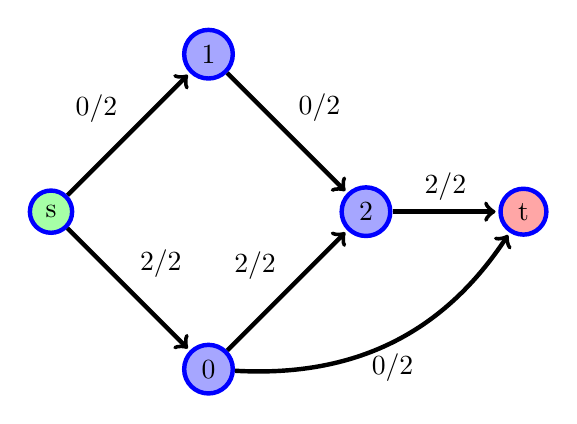
\begin{tikzpicture}[shorten >=1pt, auto, node distance=3cm, ultra thick]
   \begin{scope}[every node/.style={circle,draw=blue,fill=blue!35!}]
    \node (v1) [fill=green!35!]  at (0,2) {s};
    \node (v2) [fill=red!35!] at (6,2) {t};
    \node (v3) at (2,0) {0};
    \node (v4) at (2,4) {1};
    \node (v5) at (4,2) {2};
   \end{scope}
   \begin{scope}[->,every edge/.style={draw=black,ultra thick}]
    \draw  (v1) edge node{2/2} (v3);    
    \draw  (v1) edge node{0/2} (v4);
    \draw  (v3) edge node{2/2} (v5);
    \draw  (v4) edge node{0/2} (v5);
    \draw  (v5) edge node{2/2} (v2);
    \draw  (v3) edge [bend right, below] node{0/2} (v2);
   \end{scope}
\end{tikzpicture}
\hspace{+15mm}
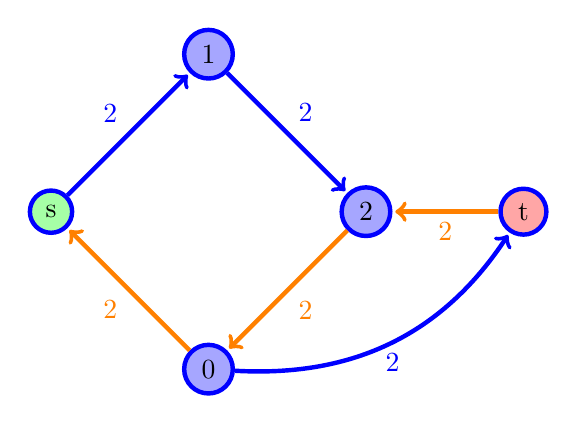
\begin{tikzpicture}[shorten >=1pt, auto, node distance=3cm, ultra thick]
   \begin{scope}[every node/.style={circle,draw=blue,fill=blue!35!}]
    \node (v1) [fill=green!35!]  at (0,2) {s};
    \node (v2) [fill=red!35!] at (6,2) {t};
    \node (v3) at (2,0) {0};
    \node (v4) at (2,4) {1};
    \node (v5) at (4,2) {2};
   \end{scope}
   \begin{scope}[->,every edge/.style={draw=black,ultra thick}]
    \draw  (v3) edge [orange] node{2} (v1);    
    \draw  (v1) edge [blue] node{2} (v4);
    \draw  (v5) edge [orange] node{2} (v3);
    \draw  (v4) edge [blue] node{2} (v5);
    \draw  (v2) edge [orange] node{2} (v5);
    \draw  (v3) edge [blue, bend right, below] node{2} (v2);
   \end{scope}
\end{tikzpicture}
\caption{An example flow network + flow is given on the left. On the right, the residual graph corresponding to this flow network + flow combo. Blue edges are forward edges and orange edges are reverse.}

\end{figure}
\end{center}
\begin{center}
\begin{figure}[!ht]
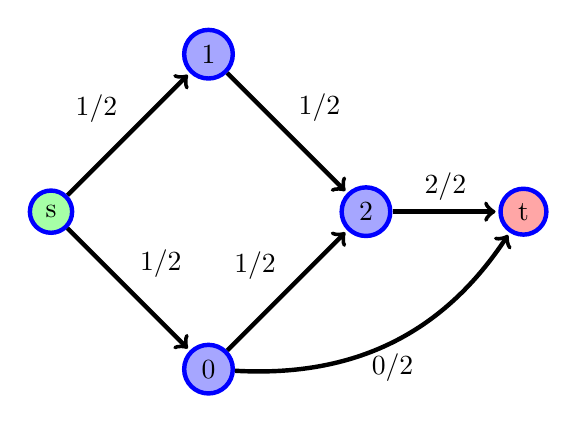
\begin{tikzpicture}[shorten >=1pt, auto, node distance=3cm, ultra thick]
   \begin{scope}[every node/.style={circle,draw=blue,fill=blue!35!}]
    \node (v1) [fill=green!35!]  at (0,2) {s};
    \node (v2) [fill=red!35!] at (6,2) {t};
    \node (v3) at (2,0) {0};
    \node (v4) at (2,4) {1};
    \node (v5) at (4,2) {2};
   \end{scope}
   \begin{scope}[->,every edge/.style={draw=black,ultra thick}]
    \draw  (v1) edge node{1/2} (v3);    
    \draw  (v1) edge node{1/2} (v4);
    \draw  (v3) edge node{1/2} (v5);
    \draw  (v4) edge node{1/2} (v5);
    \draw  (v5) edge node{2/2} (v2);
    \draw  (v3) edge [bend right, below] node{0/2} (v2);
   \end{scope}
\end{tikzpicture}
\hspace{+15mm}
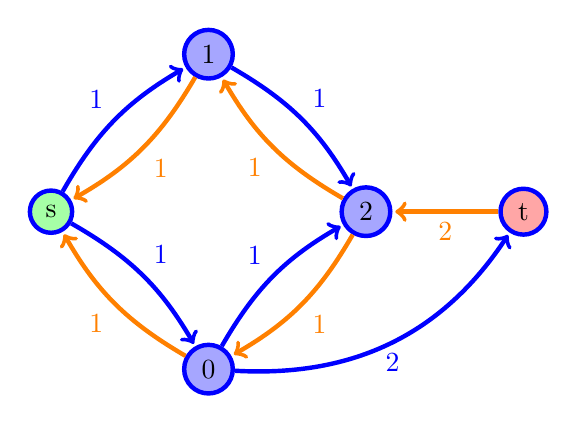
\begin{tikzpicture}[shorten >=1pt, auto, node distance=3cm, ultra thick]
   \begin{scope}[every node/.style={circle,draw=blue,fill=blue!35!}]
    \node (v1) [fill=green!35!]  at (0,2) {s};
    \node (v2) [fill=red!35!] at (6,2) {t};
    \node (v3) at (2,0) {0};
    \node (v4) at (2,4) {1};
    \node (v5) at (4,2) {2};
   \end{scope}
   \begin{scope}[->,every edge/.style={draw=black,ultra thick}]
    \draw  (v3) edge [orange, bend left=15] node{1} (v1);    
    \draw  (v1) edge [blue, bend left = 15] node{1} (v3);    
    \draw  (v1) edge [blue, bend left = 15] node{1} (v4);
    \draw  (v4) edge [orange, bend left = 15] node{1} (v1);
    \draw  (v4) edge [blue, bend left = 15] node{1} (v5);
    \draw  (v5) edge [orange, bend left = 15] node{1} (v4);
    
    \draw  (v5) edge [orange, bend left=15] node {1} (v3);
    \draw  (v3) edge [blue, bend left=15]  node{1} (v5);
    
    \draw  (v2) edge [orange] node{2} (v5);
    \draw  (v3) edge [blue, bend right, below] node{2} (v2);
   \end{scope}
\end{tikzpicture}
\caption{Here is another example. In this case, both forward and reverse edges are exemplified.}

\end{figure}
\end{center}

\begin{center}
\begin{figure}[!ht]
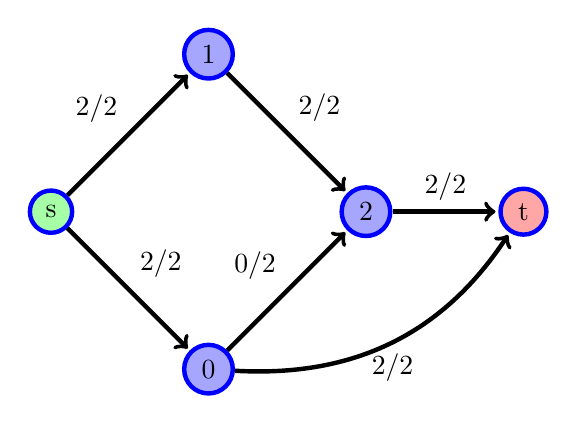
\begin{tikzpicture}[shorten >=1pt, auto, node distance=3cm, ultra thick]
   \begin{scope}[every node/.style={circle,draw=blue,fill=blue!35!}]
    \node (v1) [fill=green!35!]  at (0,2) {s};
    \node (v2) [fill=red!35!] at (6,2) {t};
    \node (v3) at (2,0) {0};
    \node (v4) at (2,4) {1};
    \node (v5) at (4,2) {2};
   \end{scope}
   \begin{scope}[->,every edge/.style={draw=black,ultra thick}]
    \draw  (v1) edge node{2/2} (v3);    
    \draw  (v1) edge node{2/2} (v4);
    \draw  (v3) edge node{0/2} (v5);
    \draw  (v4) edge node{2/2} (v5);
    \draw  (v5) edge node{2/2} (v2);
    \draw  (v3) edge [bend right, below] node{2/2} (v2);
   \end{scope}
\end{tikzpicture}
\hspace{+15mm}
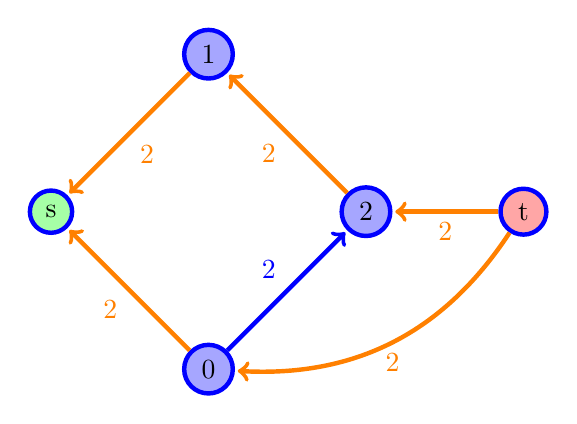
\begin{tikzpicture}[shorten >=1pt, auto, node distance=3cm, ultra thick]
   \begin{scope}[every node/.style={circle,draw=blue,fill=blue!35!}]
    \node (v1) [fill=green!35!]  at (0,2) {s};
    \node (v2) [fill=red!35!] at (6,2) {t};
    \node (v3) at (2,0) {0};
    \node (v4) at (2,4) {1};
    \node (v5) at (4,2) {2};
   \end{scope}
   \begin{scope}[->,every edge/.style={draw=black,ultra thick}]
    \draw  (v3) edge [orange] node{2} (v1);    
    \draw  (v4) edge [orange] node{2} (v1);
    \draw  (v5) edge [orange] node{2} (v4);
    
    \draw  (v3) edge [blue]  node{2} (v5);
    
    \draw  (v2) edge [orange] node{2} (v5);
    \draw  (v2) edge [orange, bend left, below] node{2} (v3);
   \end{scope}
\end{tikzpicture}
\caption{In this case, the flow in the flow network on the left-hand side is the maximum flow. Notice how there are no paths from the source to the sink in the residual graph!}
\end{figure}
\end{center}
\newpage
\noindent
Notice how in figure 13 there is a path in the residual graph from the source to the sink (it's okay if the path contains reverse edges); if there is a path in the residual graph, then it means we have not achieved maximum flow yet! Take a look at figure 15 and notice how there is NO path from source to sink --- maximum flow is achieved (remember, the maximum flow in this graph is 4)! Figure 14 is similar to figure 13 in the sense that the flow is not maximum, but observe how there are both forward and reverse edges between some of the nodes.
\\\\
At this point you should be familiar with how to construct a residual graph given a flow network and a flow going through it. If the residual graph only contained blue (read: forward) edges, it should be clear that finding a path from the source to the sink would give you a path where you could push flow along; but what about these orange (read: reverse) edges? The intuition behind these reverse edges is that they allow you to remove flow that was sent along an `bad path'. (It's not entirely obvious why using reverse edges work, but what if instead we called them `redirect' edges? Can you see what these `redirect' edges do now?)
\\\\
Suppose we have a path from the source to the sink in the residual graph. This means that we're allowed to push some amount of flow from the source to the sink (by adding new flow and potentially reversing some old flow), but how do we do this? It's easy to see that, in the case of all blues, we just find the smallest edge weight along the path and add that edge weight to each of the corresponding edges in the flow network. \\\\
When we have an orange edge along our path, instead of adding this smallest edge weight to its corresponding edge in the flow network, we subtract it (after all, we're `reversing' the flow).
\begin{center}
\begin{figure}[!ht]
\label{fig:notmax}
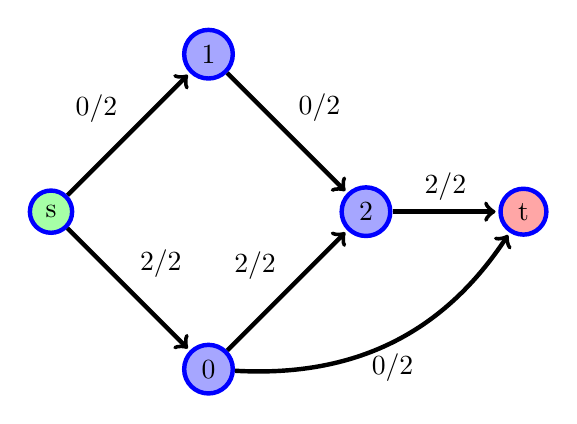
\begin{tikzpicture}[shorten >=1pt, auto, node distance=3cm, ultra thick]
   \begin{scope}[every node/.style={circle,draw=blue,fill=blue!35!}]
    \node (v1) [fill=green!35!]  at (0,2) {s};
    \node (v2) [fill=red!35!] at (6,2) {t};
    \node (v3) at (2,0) {0};
    \node (v4) at (2,4) {1};
    \node (v5) at (4,2) {2};
   \end{scope}
   \begin{scope}[->,every edge/.style={draw=black,ultra thick}]
    \draw  (v1) edge node{2/2} (v3);    
    \draw  (v1) edge node{0/2} (v4);
    \draw  (v3) edge node{2/2} (v5);
    \draw  (v4) edge node{0/2} (v5);
    \draw  (v5) edge node{2/2} (v2);
    \draw  (v3) edge [bend right, below] node{0/2} (v2);
   \end{scope}
\end{tikzpicture}
\hspace{+15mm}
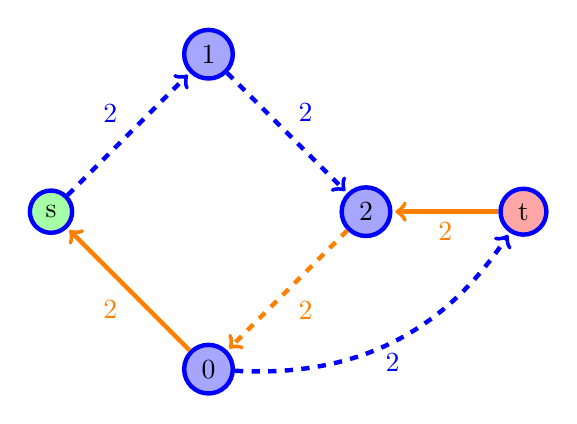
\begin{tikzpicture}[shorten >=1pt, auto, node distance=3cm, ultra thick]
   \begin{scope}[every node/.style={circle,draw=blue,fill=blue!35!}]
    \node (v1) [fill=green!35!]  at (0,2) {s};
    \node (v2) [fill=red!35!] at (6,2) {t};
    \node (v3) at (2,0) {0};
    \node (v4) at (2,4) {1};
    \node (v5) at (4,2) {2};
   \end{scope}
   \begin{scope}[->,every edge/.style={draw=black,ultra thick}]
    \draw  (v3) edge [orange] node{2} (v1);    
    \draw  (v1) edge [blue, dashed] node{2} (v4);
    \draw  (v5) edge [orange, dashed] node{2} (v3);
    \draw  (v4) edge [blue, dashed] node{2} (v5);
    \draw  (v2) edge [orange] node{2} (v5);
    \draw  (v3) edge [blue, bend right, below, dashed] node{2} (v2);
   \end{scope}
\end{tikzpicture}
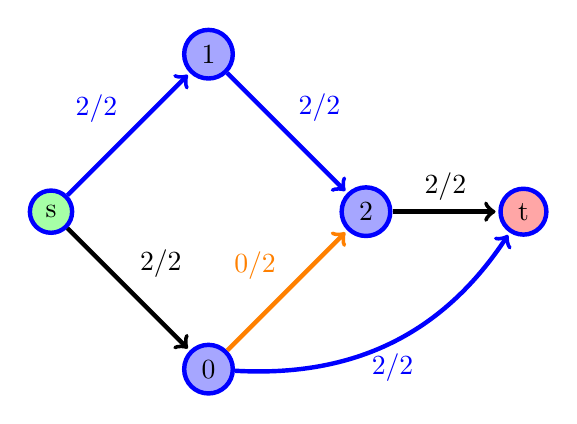
\begin{tikzpicture}[shorten >=1pt, auto, node distance=3cm, ultra thick]
   \begin{scope}[every node/.style={circle,draw=blue,fill=blue!35!}]
    \node (v1) [fill=green!35!]  at (0,2) {s};
    \node (v2) [fill=red!35!] at (6,2) {t};
    \node (v3) at (2,0) {0};
    \node (v4) at (2,4) {1};
    \node (v5) at (4,2) {2};
   \end{scope}
   \begin{scope}[->,every edge/.style={draw=black,ultra thick}]
    \draw  (v1) edge node{2/2} (v3);    
    \draw  (v1) edge [blue] node{2/2} (v4);
    \draw  (v3) edge [orange] node{0/2} (v5);
    \draw  (v4) edge [blue] node{2/2} (v5);
    \draw  (v5) edge node{2/2} (v2);
    \draw  (v3) edge [blue, bend right, below] node{2/2} (v2);
   \end{scope}
\end{tikzpicture}
\caption{A path from the source to the sink in the residual graph is shown on the right. Notice how }
\end{figure}
\end{center}
Now we're back to the situation we ended the previous section with, but are now empowered with the concept of residual graphs. Notice that along the path in the residual graph in figure 16, $2$ is the minimum edge weight, meaning we can push a flow of $2$ from the source to the sink. To achieve this we add $+2$ to each of the blue edges in the flow network and subtract $-2$ from each of the orange edges.
\\\\
It is guaranteed that doing this process of `adding/subtracting the smallest edge weight' along a path in the residual graph will result in pushing that additional amount of flow from the source to the sink. A path from the source to the sink in the residual graph is known as an \emph{augmenting path} and the process of `adding/subtracting the smallest edge weight' is known as \emph{augmenting} the flow network along this path.
\subsection{The Ford-Fulkerson algorithm}
Now it's time to use residual graphs to develop on algorithm. In fact, in the last section we had one going already:
\newpage
\noindent (0) initialize the flow in the flow network to be 0 along every edge \\
(1) find a path in the residual graph from s to t. \\
(2) `augment' this path by finding the minimum edge weight on it, adding that to the forward edges, and subtracting it from the reverse edges. \\
(3) repeat step (1) until no augmenting path exists. \\\\
Unlike the first algorithm we developed, once no path exists in the residual graph we're guaranteed that we've have the maximum flow going from the source to the sink. When step (1) is done with the depth-first search (DFS) algorithm, this is called the \emph{Ford-Fulkerson method}. The run-time of the Ford-Fulkerson method is $$\boxed{O(E |f^*|)}$$
Remember that $|f^*|$ is the maximum flow in the flow network. If we have a flow network that has a large maximum flow, the Ford-Fulkerson method runs reaaaaaaalllllllyyyy slow. We'll make a quick modification before we code it up that will vastly improve its runtime.
\subsection{The Edmonds-Karp algorithm}
Notice how in step (1) I just arbitrarily said to use depth-first search to find an augmenting path. It turns out that this is the reason the Ford-Fulkerson method is slow. Without a proof or any sort of intuition behind it (it's honestly not worth the trouble) I'm going to claim that using breadth-first search (BFS) will change the run-time of the previous algorithm to $$\boxed{O(V^2E)}$$
This is much better for the majority of cases and so it will be the algorithm we implement.
\subsection{Implementing Edmonds-Karp}
The idea is fairly simple after we went through all of it, but how do we code it? There are a \emph{ton} of ways to implement these algorithms. In the following implementation we assume that there is at most one edge between two nodes in the flow network provided. As with most graph algorithms, we assume that the vertices are numbered between $[0, n-1]$ for some $n$. In addition, for this code to work, we assume that there is at most one edge between any pair of nodes in the flow network given. 
\\\\
TODO: MORE EXPLANATION MAYBE?
\begin{lstlisting}
class EdmondsKarp {
	//capacity[i][j] = the capacity of the edge going from i to j
	int[][] capacity;

	//flow[i][j] = the flow going from i to j
	//0 <= flow[i][j] <= capacity[i][j]
	int[][] flow;

	//the number of nodes in our graph.
	int N;

	public EdmondsKarp(int numNodes) {
		this.capacity = new int[numNodes][numNodes];
		this.flow = new int[numNodes][numNodes];
		this.N = numNodes;
	}

	//add an edge going from `from' to `to'
	//with capacity `cap'
	//note that this code FAILS when a pair of nodes
	//have two edges between them
	void addEdge(int from, int to, int cap) {
		capacity[from][to] = cap;
		flow[from][to] = 0;
	}

	//compute the maximum flow from `src' to `snk'
	int maxflow(int src, int snk) {
		int maximum_flow = 0;
		while (true) {
			//step (1) find an augmenting path
			int[] path = find_path(src, snk);

			//stop if no augmenting path exists!
			if (path == null) break;

			//step (2) augment the path
			maximum_flow += augment(path);

			//step (3) rinse and repeat
			continue;
		}
		return maximum_flow;
	}

	//find_path finds an augmenting path (in the residual graph)
	//from `src' to `snk'
	//if a path exists, we return it as a sequence of the vertices
	//we find the path with breadth-first search.
	int[] find_path(int src, int snk) {
		Queue<Integer> q = new LinkedList<Integer>();
		//pred[i] stores the predecessor of node i
		//along its shortest path from src to snk.
		int[] pred = new int[N];
		q.add(src);
		//-1 means it is the src, -2 means it hasnt been visited
		Arrays.fill(pred, -2);
		pred[src] = -1;
		while (!q.isEmpty()) {
			int front = q.poll();
			for (int next = 0; next < N; next++) {
				//check if we can move go along (front->next)
				//edge in the residual graph
				//we can move along this edge iff:
				//it's a blue edge: (capacity[front][next]-flow[front][next] > 0)
				//it's an orange edge: (flow[next][front] > 0)
				//notice for the orange edge we check flow[next][front]
				//(the reverse)
				if ((capacity[front][next]-flow[front][next]) > 0 
					|| flow[next][front] > 0) {
					//we need to make sure we havent visited `next' yet!
					if (pred[next] == -2) {
						q.add(next);
						pred[next] = front;
					}
				}
			}
		}
		//snk wasnt visited...there is no path to it!
		if (pred[snk] == -2) {
			return null;
		}
		//the path is stored in reverse, so we use
		//a stack to order it properly
		Stack<Integer> path = new Stack<Integer>();
		int cur = snk;
		while (true) {
			path.add(cur);
			cur = pred[cur];
			if (cur == -1) break;
		}
		int[] array_path = new int[path.size()];
		int idx = 0;
		while (!path.isEmpty()) {
			array_path[idx++] = path.pop();
		}
		return array_path;
	}

	//augment the path (add/subtract the minimum edge weight)
	//along the path depending on the edges color
	//`path' is given as a sequence of vertices along the path
	//we return the amount of flow we send from the source to the sink
	int augment(int[] path) {
		int min_edge_weight = Integer.MAX_VALUE;
		//first we find the minimum edge weight on this path:
		for (int i = 0; i < path.length-1; i++) {
			int from = path[i];
			int to = path[i+1];
			int test_forward = capacity[from][to] - flow[from][to];
			int test_reverse = flow[to][from];
			//only one of these is true
			//if it's the first one, then this is a blue edge
			//if the second one is, then it's an orange edge
			if (test_forward > 0) {
				min_edge_weight = Math.min(min_edge_weight, test_forward);
			} else if (test_reverse > 0) {
				min_edge_weight = Math.min(min_edge_weight, test_reverse);
			}
		}
		for (int i = 0; i < path.length-1; i++) {
			int from = path[i];
			int to = path[i+1];
			int test_forward = capacity[from][to] - flow[from][to];
			int test_reverse = flow[to][from];
			if (test_forward > 0) {
				//if its a forward edge, we add to flow[from][to]:
				flow[from][to] += min_edge_weight;
			} else if (test_reverse > 0) {
				//if its a reverse edge, we subtract from flow[to][from]:
				flow[to][from] -= min_edge_weight;
			}
		}
		//we just sent `min_edge_weight' flow from the source 
		//to the sink
		return min_edge_weight;
	}
}
\end{lstlisting}
%define largest valid flow
%show what it looks like?
%'augmenting path' idea.
%ford fulkerson	
%edmonds karp
%code
\section{Some useful reductions}
Remember the idea of \emph{reduction} that we talked about in the introduction? We'll be applying the idea of maximum flow to solve other seemingly unrelated graph problems. To do this, we're going to try and cast our new problem in terms of a flow network where the answer is the maximum flow.
\subsection{Maximum Cardinality Bipartite Matching}
Now we're going to take a look at the \emph{maximum cardinality bipartite matching problem} or more commonly referred to as the \emph{job assignment problem}. Imagine you're given a set of job applicants and a set of jobs. Each job applicant has a certain skill set and therefore can only apply to certain jobs. Under the assumption that a person can only work one job and a job can only be worked by one person, what is the maximum amount of job assignments that we can make? Below is an example situation where we're given the job applicants, the jobs, and we draw an edge between the job applicant and job if he/she is qualified for the job; the best assignment is colored in red.
\begin{figure}[!ht]
\centering
\caption{An example job assignment scenario modeled as a graph problem. The edges that correspond to a maximum matching are highlighted in red.}
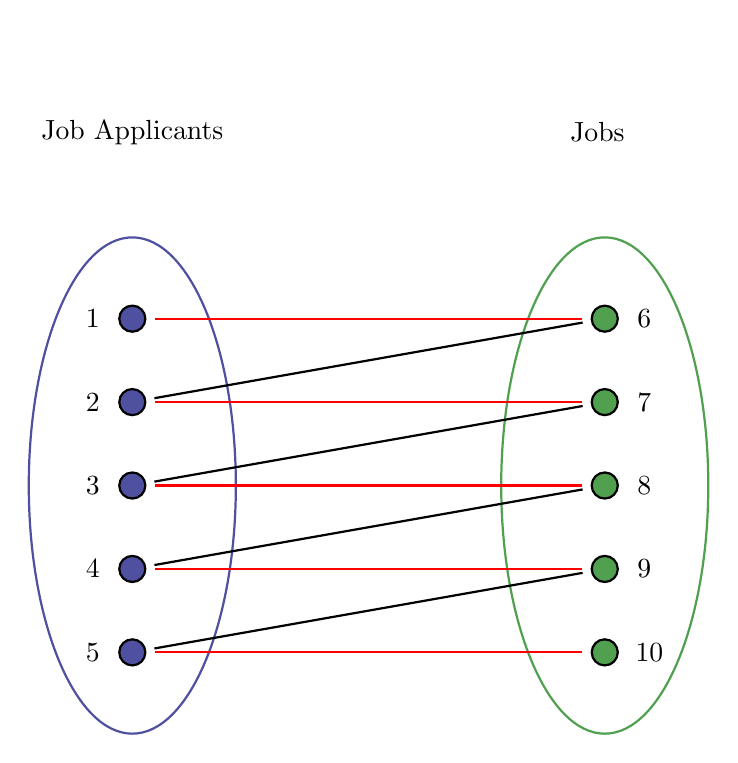
\begin{tikzpicture}[thick,
  every node/.style={draw,circle},
  fsnode/.style={fill=myblue},
  ssnode/.style={fill=mygreen},
  every fit/.style={ellipse,draw,inner sep=-2pt,text width=2cm},
  shorten >= 3pt,shorten <= 3pt
]

% the vertices of U
\begin{scope}[start chain=going below,node distance=7mm]
\foreach \i in {1,2,...,5}
  \node[fsnode,on chain] (f\i) [label=left: \i] {};
\end{scope}

% the vertices of V
\begin{scope}[xshift=6cm, start chain=going below,node distance=7mm]
\foreach \i in {6,7,...,9, 10}
  \node[ssnode,on chain] (s\i) [label=right: \i] {};
\end{scope}

% the set U
\node [myblue,fit=(f1) (f5),label=above:Job Applicants] {};
% the set V
\node [mygreen,fit=(s6) (s10),label=above:\phantom{xxxx}Jobs\phantom{xxxxx}] {};

% the edges
\draw [red] (f1) -- (s6);
\draw (f2) -- (s6);
\draw [red] (f2) -- (s7);
\draw (f3) -- (s7);
\draw [red] (f3) -- (s8);
\draw (f4) -- (s8);
\draw [red] (f4) -- (s9);
\draw (f5) -- (s9);
\draw [red] (f5) -- (s10);
\end{tikzpicture}
\end{figure}
\newpage \noindent Take a moment to think about this problem. Can you see the similarities with max flow? Specifically, if we try and take an `incremental' approach like we did initially with max flow, we have the potential to get a `bad match' (remember `bad paths'?) and then get stuck. We will use our maximum flow algorithm to fix this issue.
\\\\
\noindent TODO: DO THIS
%bipartite matching
%edge disjoint paths?
%vertex disjoint paths?
\section{Taking it a step further: cuts and duality}
%define s-t cut
%show examples of s-t cut
%minimum s-t cut
%min st cut is like the 'bottle neck' for flow 
%min st cut == max flow
\section{EXAMPLE OF USEFULNESS OF CUTS}
%???
\section{Comments}
%global cuts
%dinitz
%relabel flow
%hopcroft karp/augmenting path algos
%closure problem
\section{Problems}
$$\boxed{\text{http://www.spoj.com/problems/POTHOLE/}}$$
\section*{Code Appendix}
\end{document}
